\documentclass[12pt]{article} % velikost písma a typ dokumentu
\usepackage[utf8]{inputenc}  % kódování
\usepackage[czech]{babel}  % jazykový balík
\usepackage{graphicx}  % balik nutný pro vkládání obrázků
\usepackage{indentfirst}  % odsazení prvního řádku v odstavci (někdy se to dělá, někdy ne - co je správně nevím)
\usepackage{amsmath}
\usepackage{float}
\usepackage{caption}
\usepackage{url}

\usepackage{listings}
\usepackage[T1]{fontenc}
\usepackage{csquotes}
\usepackage[backend=biber, style=iso-numeric]{biblatex}
\addbibresource{citations.bib}
\renewcommand{\thesubsection}{\thesection.\alph{subsection}} % číslování 1.a 1.b ....

\begin{document}  % začátek dokumentu - na konci je end ;)

\begin{figure}[h!] % vkládání plovoucího prostředí pro obrázky parametr, vynucuje umístění here!
\centering % zajištění centrování - pro aktuální 'figure'

\includegraphics[width=0.4\textwidth]{pic/FAV_cmyk.png} % vložení obrázku - i s cestou jeho umístění !
\hspace{2cm}  % vložení horizontální mezery

\includegraphics[width=0.4\textwidth]{pic/KKY_logo_cz_large.png} % vložení obrázku
\end{figure}

\begin{center} % centrování textu (begin - end)

\LARGE{Semestrální práce z předmětu LS1}\\ % lokální modifikace velikosti textku (relativně k definici v documentclass)
\large{Návrh systému automatického řízení teploty}
\vspace{.5cm} % vložení vertikální mezery
\end{center}


\vfill{}  % vyplnění 'prázdnem' - zajistí, že zbytek bude dole na stránce 
\noindent  % zabrání odsazení nového odsatvce
Západočeská Univerzita V Plzni \hfill Martin Rob \\  % vyplnění prázdnem - horizontální
Katedra Kybernetiky \hfill Lukáš Egr\\
Semestrální práce - LS1 \hfill \today % today vypíše datum - ve formátu definovaném volbou jazyka. 
\thispagestyle{empty}  % zakáže číslování stránky
\newpage % zalomení stránky
\setcounter{page}{1} % nastaví počítadlo stránek

\section{Seznámení s modelem teplotního systému TClab}
\subsection{Popis struktury systému z pohledu řízení}
Systém se skládá ze dvou topných těles, a dvou senzorů teploty. Konkrétně setTopná tělesa skládají z tranzistorů (TIP31C) a na nich umístěných chladičů, výsledná teplota je pak měřená teplotními senzory (TMP36). Jednotlivá topná tělesa lze řídit jednotlivě.

Z pohledu řízení má systém dva vstupy (výkony jednotlivých topení) a dva výstupy (naměřené teploty). Neboli naše měřené veličiny jsou aktuální teploty a akční veličiny jsou výkony jednotlivých topnách těles.

\subsection{Fyzikální paramtery systému}
Fyzikální parametry systému, které budou ovlívňovat dynamiku systému jsou následující

\begin{itemize}
    \item \textbf{Tepelná kapacita:} Hmotnost topného tělesa a jeho měrná tepelná kapacita ($m \cdot c_p$) nám určuje ovlivňujě, jak rychle/pomalu se tělesa zahřívají/chladnou.
    
    \item \textbf{Odvod tepla do okolí:} Povrch tělesa ($A$), odkud teplo odchází do okolí, součinitel přestupu tepla prouděním ($U$) a emisivita ($\epsilon$), která ovliňujew ztráty tepelným zářením.
     
    \item \textbf{Vzájemné ovliňiování:} Interakční plocha obou těles ($A_{int}$), která určuje jak rychle se teplo přenáší mezi tělesy.
    
    \item \textbf{Výkon topných těles} Vstupní výkon obou těles ($Q_1$ a $Q_2$).
\end{itemize}

\section{Matematický model systému}
\subsection{Odvození pohybové rovnice systému s jedním tělesem}
Abychom odvodili pohybovou rovnici systému musíme nejdříve porozumět výchozí rovnici, vycházející z 1. termodynamického zákona o zachování energie v otevřeném systému

\begin{equation}
    \label{eq:tclab}
    m c_p \frac{dT}{dt} = \sum \dot{m}_{in} c_p (T_{in} - T_{ref}) - \sum \dot{m}_{out} c_p (T_{out} - T_{ref}) + Q + W_s,
\end{equation}

kde m je hmotnost ohřívacího tělesa, $c_p$ měrná tepelná kapacita topného tělesa, $\dot{m}_{in}$~hmotnostní tok média k tělesu, $\dot{m}_{out}$~hmotnostní tok média od tělesa, $T_{in}$~vstupní teplota, $T_{ref}$~teplota v místnosti/referenční teplota, Q celkový výkon systému a $W_s$ je vstupní externí práce. V našem případě žádné protékající médium nepoužíváme. Zároveň žádnou vnější práci so systému nepřidáváme. Pohybovou rovnici lze zredukovat na jednodušší tvar (viz rovnice \ref{eq:zredTclab}).

\begin{equation}
    \label{eq:zredTclab}
    m c_p \frac{dT}{dt} = Q 
\end{equation}

Nyní si lze vyjádřit celkový výkon systému jako kombinaci výkonu topného tělesa a jeho ztrát.
U našeho topného tělesa uvažujeme dvě hlavní ztráty energie: ztráta prouděním (konvekcí) a vyzářením (emisí). Po dosazení získáme pravou stranu rovnice

\begin{equation}
    \label{eq:pravStranaZredTclab}
    Q_T - Q_e - Q_p,
\end{equation}

kde $Q_T$ je výkon topného tělesa, $Q_e$ výkon, který se vyzáří emisí a $Q_p$ je výkon, který se ztratí ochlazováním prouděním vzduchu kolem tělesa. Po dosazení získáme pohybovou rovnici pro jedno těleso

\begin{equation}
    \label{eq:pohRov}
    m c_p \frac{dT}{dt} =  Q_T - \varepsilon \sigma S (T^4 - T_{ref}^4) - U S (T - T_{ref}),
\end{equation}
kde S je plocha topného tělesa, $\varepsilon$ emisivita, $\sigma$ Stefan-Boltzmannova konstanta a U je součinitel prostupu tepla.
\subsection{Rozhodnutí (ne)linearity systému}
Lineární systémy jsou charakteristické principem superpozice. U našeho systému s pohybovou rovnicí v tomto tvaru (viz rovnice \ref{eq:pohRov}) princip neplatí. Důvodem je člen ztrát emisí, kde se nachází čtvrtá mocnina teploty a také nenulové konstantní členy teploty okolí($T_ref$).
\subsection{Simulační model}
Pro namodelování v softwaru Simulink, je nutné z pohybové rovnice (viz \ref{eq:pohRov}) vyjádřit derivaci teploty.
\begin{equation}
    \label{eq:matModel}
    \frac{dT}{dt} =  \frac{1}{m c_p}\left(Q_T - \varepsilon \sigma S (T^4 - T_{ref}^4) - U S (T - T_{ref})\right),
\end{equation}
Abychom upravenou rovnici mohli vložit do bloku MatLab funkce (viz obrázek \ref{fig:simlModPR}), je nutné zápis přeložit do matlab kódu.

\begin{lstlisting}[language=MatLab]
function out = fcn(m,c_p,U,area,Q_in,T_ok,sigma,epsilon,T)
    out = (1/(m*c_p))*(Q_in - U*area*(T-T_ok) 
    - sigma*epsilon*area*((T^4)-(T_ok^4)));
\end{lstlisting}
Na výstup modelu pohybové rovnice (předchozí matlab funkce), tedy derivaci teploty, je nutné použít integrátor s poč. podmínkou $T_{(0)}=T_{\text{okolí}}=293.15 \text{K}$. Integrací získáme teplotu $\text{T}$, kterou přivedeme na příslušný vstup.
\begin{figure}[htbp]
    \centering
    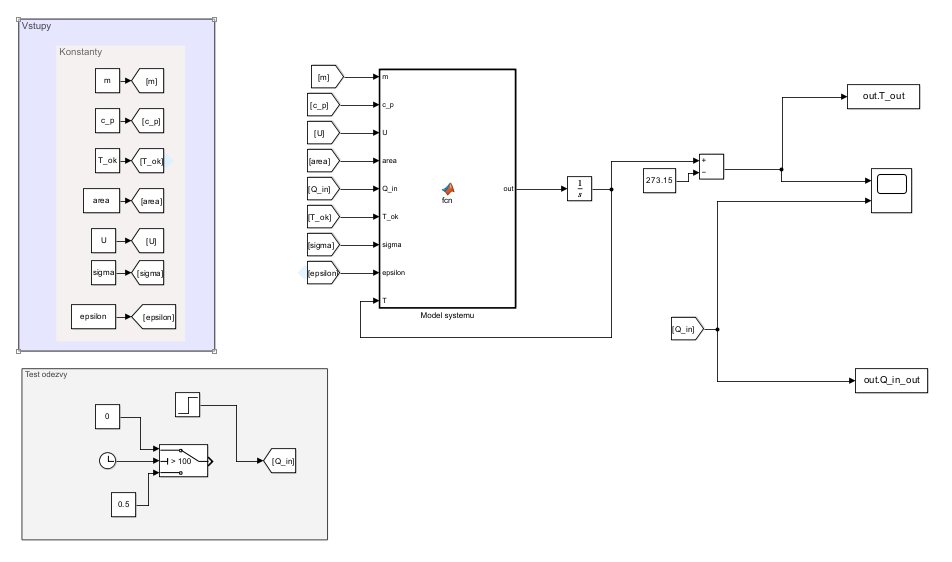
\includegraphics[width=0.7\textwidth]{pic/mat_model_jednoTeleso.png}
    \caption{Blokový popis pohybové rovnice v softwaru Simulink}
    \label{fig:simlModPR}
\end{figure}

\newpage

\subsection{Fyzikální parametry}
Hodnoty konstant a veličin byly získány z webu TCLab \cite{apmonitor_tclab}
\begin{table}[htbp]
    \centering
    \caption{Přehled fyzikálních parametrů a konstant modelu.}
    \label{tab:fyz_parametry}
    \begin{tabular}{llcl}
        \hline
        \textbf{Parametr} & \textbf{Název veličiny / konstanty} & \textbf{Hodnota} & \textbf{Jednotka} \\
        \hline
        $m$ & Hmotnost ohřívacího tělesa & $0{,}004$ & $\mathrm{kg}$ \\
        $c_p$ & Měrná tepelná kapacita tělesa & $500$ & $\mathrm{J \cdot kg^{-1} \cdot K^{-1}}$ \\
        $S$ & Plocha povrchu tělesa & $0{,}0012$ & $\mathrm{m^2}$ \\
        $U$ & Součinitel prostupu tepla (konvekce) & $10$ & $\mathrm{W \cdot m^{-2} \cdot K^{-1}}$ \\
        $\varepsilon$ & Emisivita povrchu tělesa & $0{,}9$ & $-$ \\
        $\sigma$ & Stefan-Boltzmannova konstanta & $5{,}670374 \cdot 10^{-8}$ & $\mathrm{W \cdot m^{-2} \cdot K^{-4}}$ \\
        $T_{\mathrm{ok}}$ & Počáteční a okolní teplota ($20\,^\circ\mathrm{C}$) & $293{,}15$ & $\mathrm{K}$ \\
        \hline
    \end{tabular}
\end{table}

\begin{figure}[h!]
    \centering
    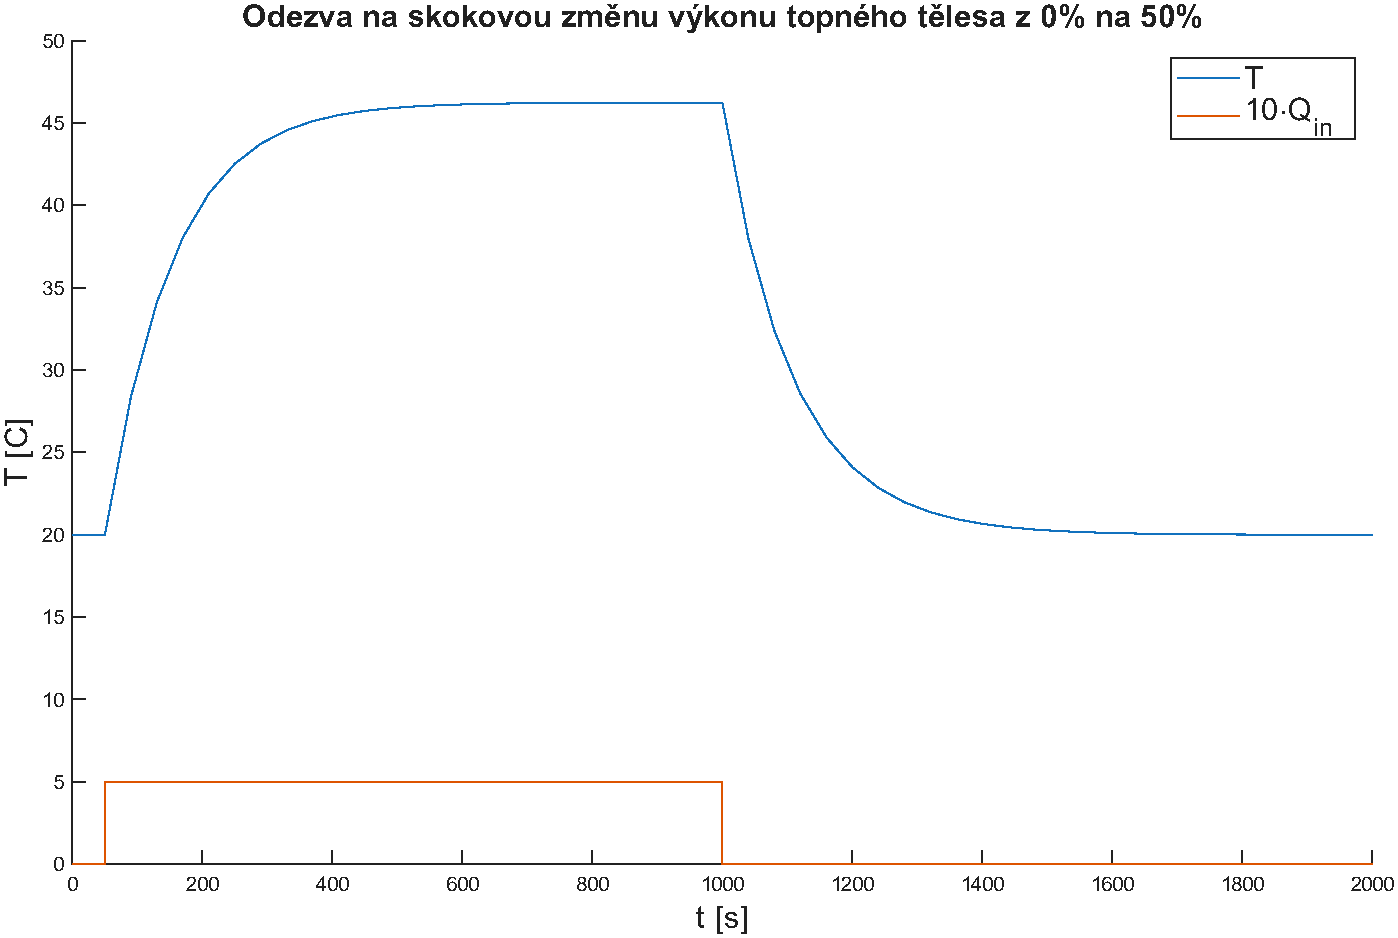
\includegraphics[width=0.9\textwidth]{pic/odezva_2d.pdf}
    \caption{Průběh odezvy na skokovou změnu vstupu tělesa}
    \label{g:odezvaNa50Vykon}
\end{figure}

Odezva systému (viz Obrázek \ref{g:odezvaNa50Vykon}) je aperiodická a stabilní. Ze začátku náběhu výkonu je patrné, že systém žádný inflexní bod nemá a tedy jde o odezvu 1. řádu.Teplota systému se ustálila v novém pracovním bodě~$\approx 46,3^\circ\text{C}$. V grafu jsou hodnoty $Q_{in}$ pro lepší přehlednost desetinásobné.

\subsection{Převažující ztráty}
Je nutné zjistit, jaké ztráty převažují v pracovních podmínkách našeho tělesa ($20-100 ^\circ \text{C}$). Je patrné, že kvůli malé hodnotě Stefan-Boltzmannovy konstanty se pro menší hodnoty teploty bude nejvíce podílet ztráta prouděním. Nalezneme teplotní bod kdy ztráty emisí budou ekvivalentní se ztrátami prouděním.
\begin{equation*}
    U S (T-T_{ok}) = S \varepsilon \sigma (T^4 - T_{ok}^4)
\end{equation*}
Dosadíme hodnoty z tabulky \ref{tab:fyz_parametry}.
\begin{equation*}
    \varepsilon \sigma \approx 5,1 \cdot 10^{-8}
\end{equation*}

\begin{equation*}
    10 (T-T_{ok}) = 5,1 \cdot 10^{-8} (T^4 - T_{ok}^4)
\end{equation*}

\begin{equation*}
    10 (T-T_{ok}) = 5,1 \cdot 10^{-8} (T^2 - T_{ok}^2) (T^2 + T_{ok}^2)
\end{equation*}

\begin{equation*}
    10 (T-T_{ok}) = 5,1 \cdot 10^{-8} (T - T_{ok}) (T + T_{ok}) (T^2 + T_{ok}^2)
\end{equation*}

\begin{equation*}
    10 = 5,1 \cdot 10^{-8} (T + T_{ok}) (T^2 + T_{ok}^2)
\end{equation*}

\begin{equation*}
    \frac{10}{5,1 \cdot 10^{-8}} = (T + T_{ok}) (T^2 + T_{ok}^2)
\end{equation*}

\begin{equation*}
    \frac{10}{5,1 \cdot 10^{-8}} = 1,96 \cdot 10^{8}
\end{equation*}

\begin{equation*}
    0 = T^3 + 2 \cdot 273,15^2 T^2 + 273,15^3 - 1,96 \cdot 10^8
\end{equation*}
S využitím online řešiče získáme hodnotu teploty, pro kterou si jsou hodnoty obou druhů ztrát rovny.
\begin{equation*}
    T = 495,4 \text{K} \approx 222 ^{\circ}\text{C}
\end{equation*}
Výsledek indikuje, že pro naše pracovní rozmezí $20-100 ^\circ \text{C}$ se nejvíce projevují ztráty prouděním.

\printbibliography
\end{document}


